\documentclass{beamer}

\usetheme{Madrid}

\usepackage{lipsum}
\usepackage{multicol}
\usepackage{listings}


% Define a custom color
\definecolor{backcolour}{rgb}{255,255,255}
\definecolor{codegreen}{rgb}{0,0.6,0}

% Define a custom style
\lstdefinestyle{myStyle}{
    backgroundcolor = \color{backcolour},   
    commentstyle = \color{codegreen},
    basicstyle=\linespread{0.4}\tiny,
    breakatwhitespace=false,         
    breaklines=true,        
    keepspaces=true,                 
    numbers=false,       
    numbersep=5pt,                  
    showspaces=false,                
    showstringspaces=false,
    showtabs=false,                  
    tabsize=2,
}

% Use \lstset to make myStyle the global default
\lstset{style=myStyle}

\usepackage{graphicx}
\usepackage{listings}
\usepackage{verbatim}
\linespread{1.5}

\usepackage{amsmath, amsthm, amssymb, latexsym}

%\newtheorem{definition}{Definition}

\newcommand{\pathtoimages}{/Users/charlesrambo/Desktop/Bootcamp24/Images}

\title{Introduction}
\author{Charles Rambo}
\institute{UCLA Anderson School of Management}
\date{2024}
\location{Los Angeles, California}

% Turn on slide numbers:
\showSlideNumber{}

\AtBeginSection[]
{
    \begin{frame}
        \frametitle{Table of Contents}
        \tableofcontents[currentsection]
    \end{frame}
}


\begin{document}
\input{systempreamble}

\insertTitleSlide

\frame{\titlepage}

\begin{frame}

\frametitle{Table of Contents}
\tableofcontents
\end{frame}

\section{Python}

\begin{frame}
\frametitle{Python Installation}
\begin{itemize}
\item We'll be using Python.
\item If you haven't used Python before, I suggest downloading Anaconda at  \url{https://www.anaconda.com/download}
\end{itemize}
\begin{center}

\includegraphics[scale = 0.1]{\pathtoimages/anaconda.png}
\end{center}
\end{frame}

\begin{frame}
\frametitle{Anaconda}

After you've installed and opened Anaconda, a screen like this will appear. You have several choices for IDEs. Spyder is useful for data analysis. Jupyter Notebook is popular for explanatory work, so students and teachers tend to use it. You can use any IDE.
\begin{center}
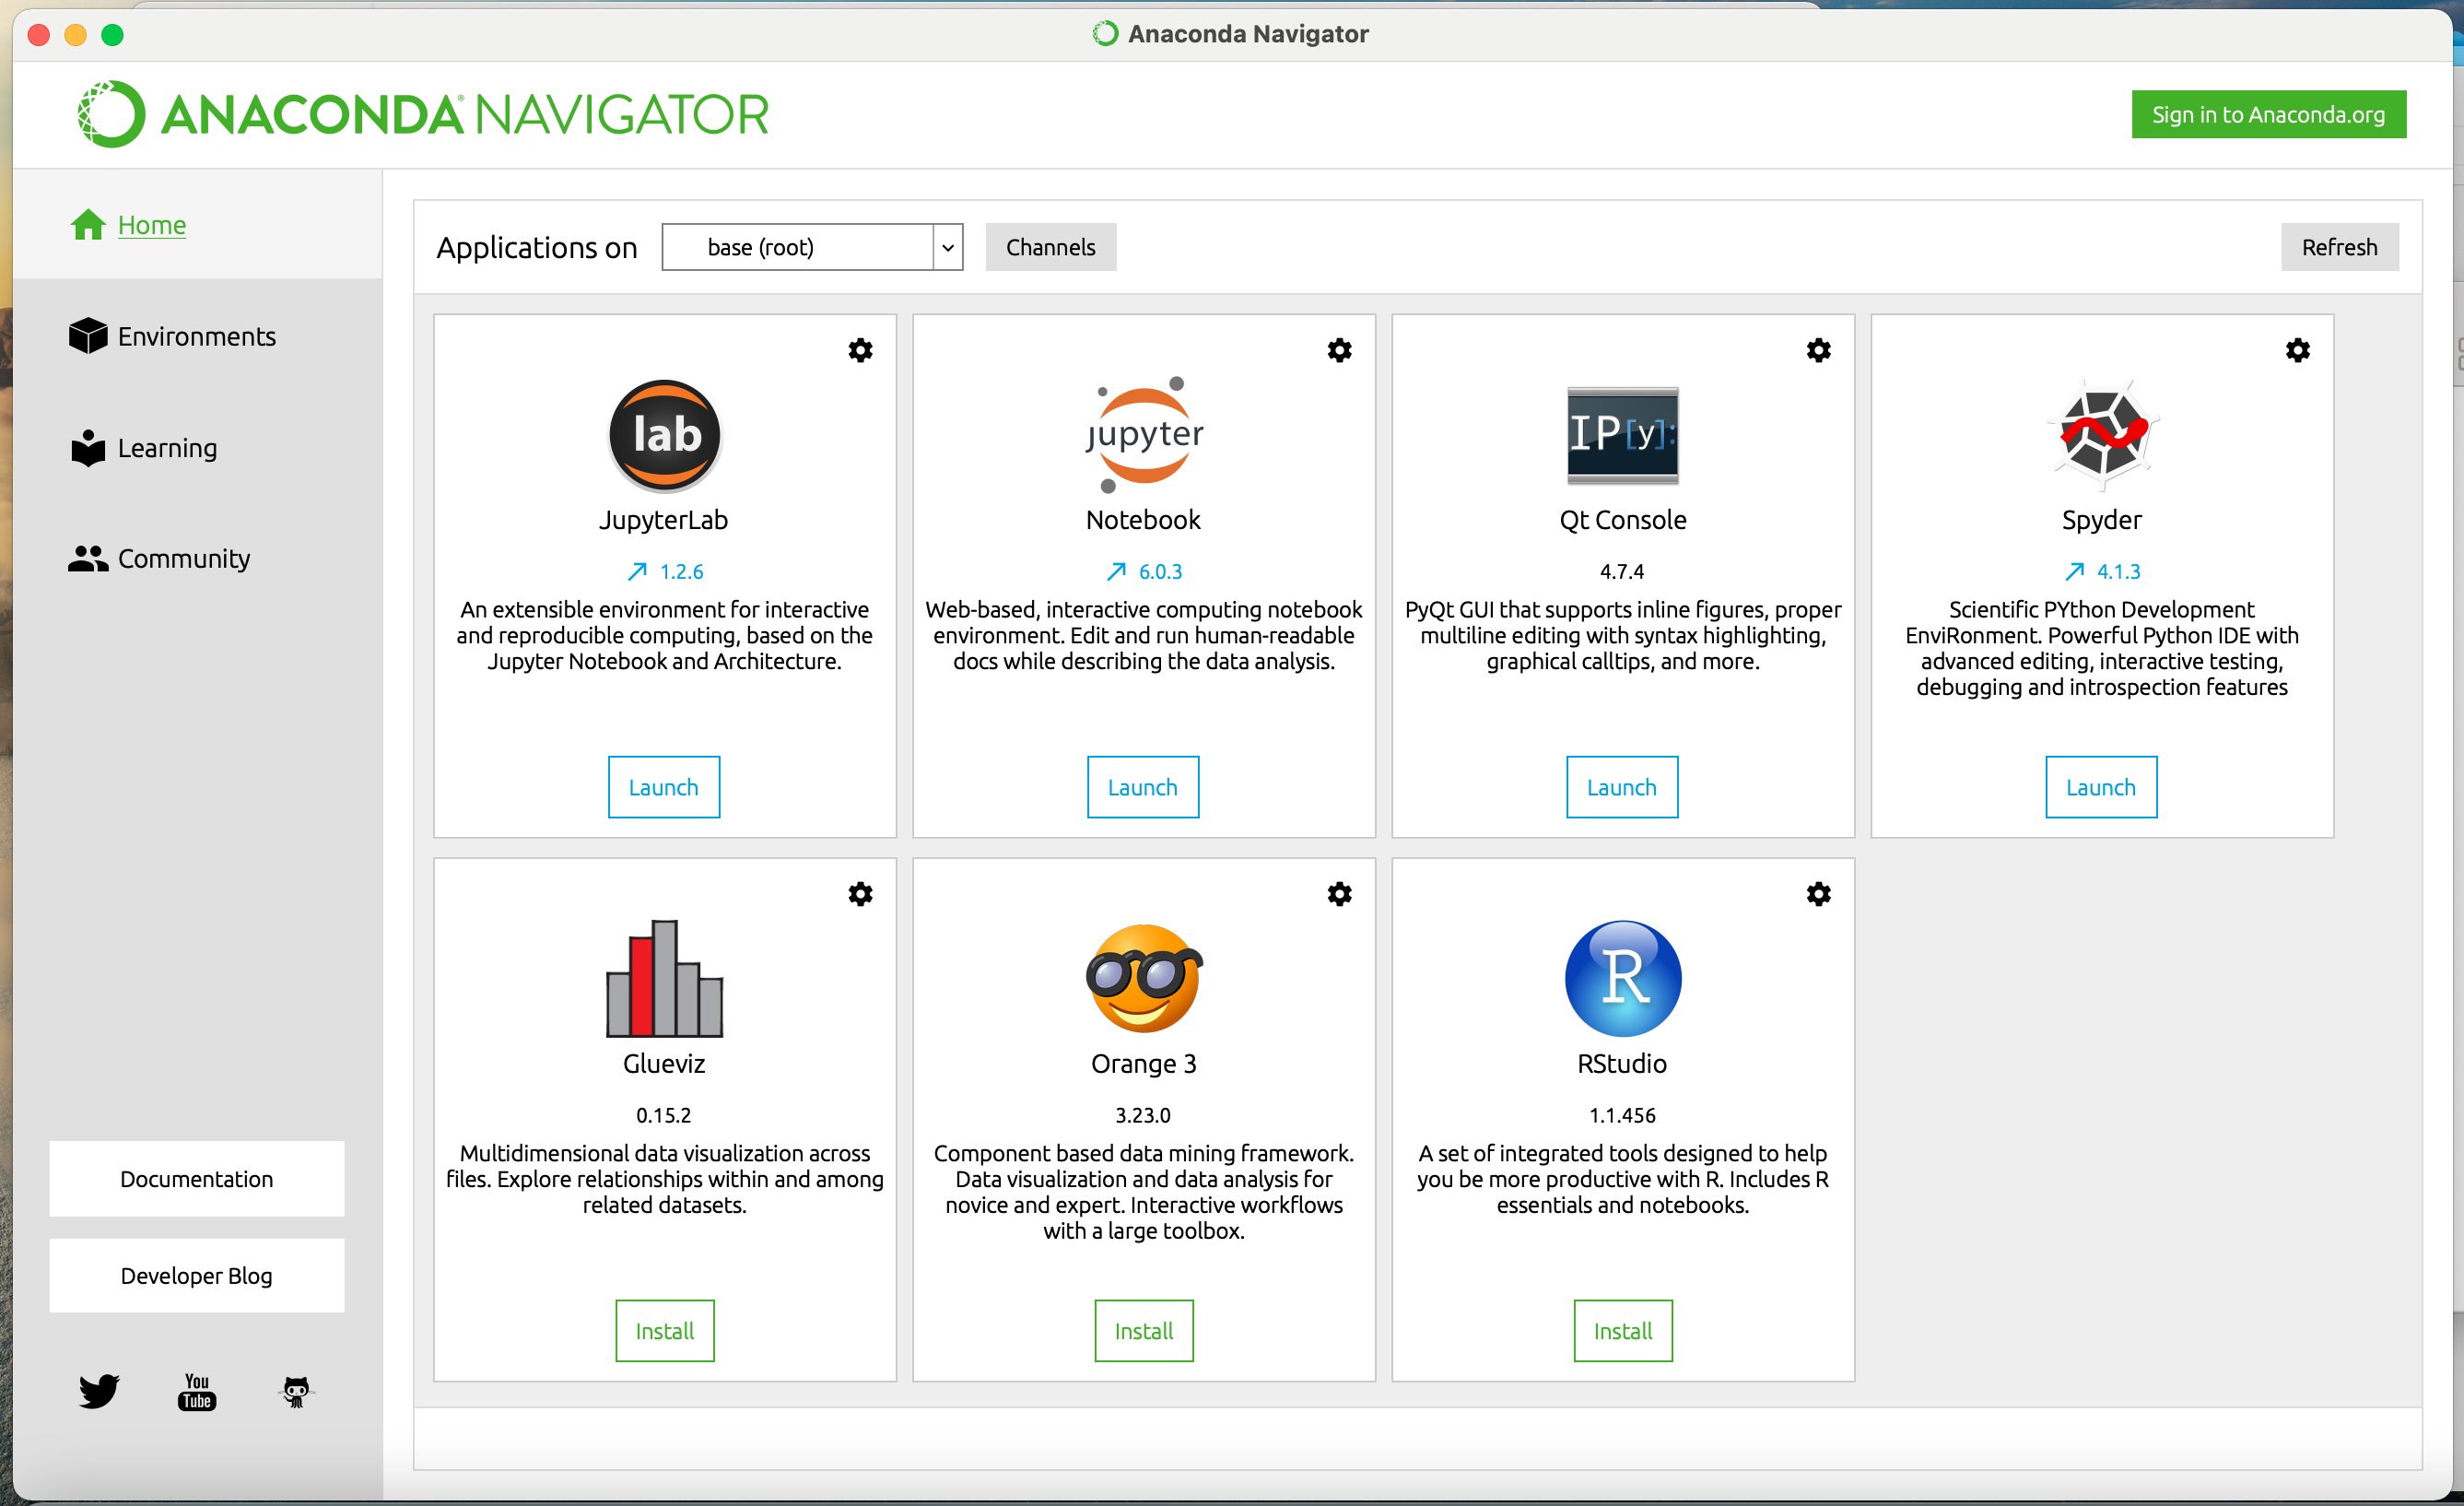
\includegraphics[scale = 0.1]{\pathtoimages/anaconda2.png}
\end{center}
\end{frame}

\frame{
\frametitle{Packages}

{
%\linespread{1.5}
Several popular modules (packages) are preinstalled in Anaconda. 
\begin{itemize}
\item {\it NumPy}:  Useful math functions.
\item {\it Matplotlib:} Graphing. Somewhat quirky syntax but very popular nonetheless. 
\item {\it SciPy}: Scientific computing functions.
\end{itemize}
}
}

\frame{
\frametitle{Package Installation} 
To install a new package, go into Terminal, and type 
\begin{center}
{\tt pip install \ldots}
\end{center}
In this example, I'm upgrading pandas. Your Terminal will probably look different.
\begin{center}
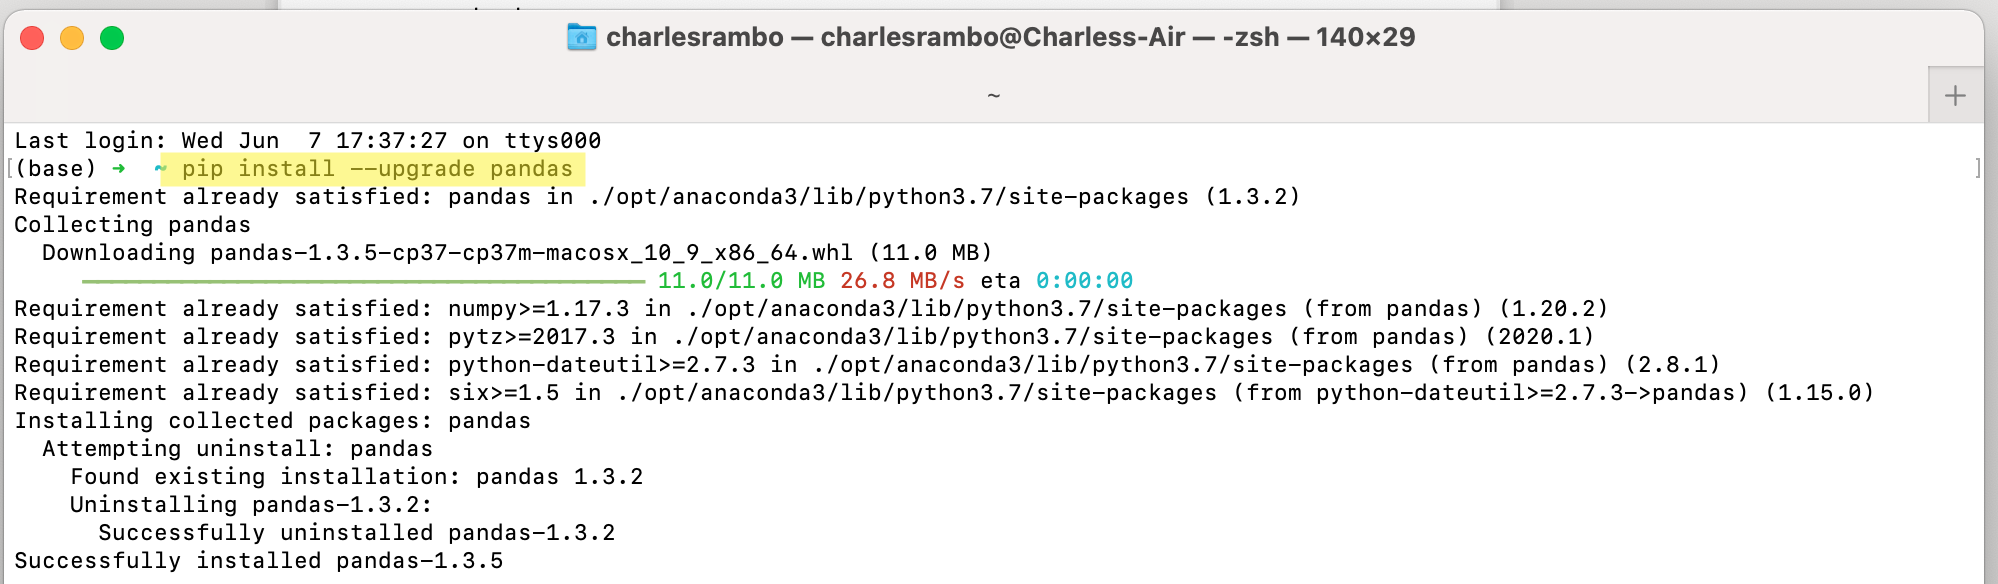
\includegraphics[scale = 0.2]{\pathtoimages/pip.png}
\end{center}
}

\begin{frame}[fragile]
\frametitle{Python Graphing Example}

\begin{example} 
Let $f(x) = x^2 + 1$. Use Python to graph $f$ on the domain $[-1, 2]$.
\end{example}

\begin{multicols}{2}
\begin{lstlisting}[language=Python]
# Import modules 
import numpy as np
import matplotlib.pyplot as plt

# These steps add style; less important

# Use latex
plt.rcParams['text.usetex'] = True

# Use Seaborn style
plt.style.use('seaborn')

# Define f
def f(x):
    return x**2 + 1

# Another option is to use a lambda function
# f = lambda x: x**2 + 1

# Get 100 x-values on [-1, 2]
x_vals = np.linspace(-1, 2, 100)

# Use list comprehension to get y-values
y_vals = [f(x) for x in x_vals]

# Generate the plot
plt.plot(x_vals, y_vals)

# Label the x-axis
plt.xlabel(r'$x$')

# Label the y-axis
plt.ylabel(r'$y$')

# Give the graph a title
plt.title(r'Graph of $y = x^2 + 1$')

# Save the figure
plt.savefig(r'[location on machine]')

# Display the plot
plt.show()

\end{lstlisting}

\end{multicols}

\end{frame}

\begin{frame}
\frametitle{Python Graphing Result}
\begin{center}
\includegraphics[scale = 0.5]{\pathtoimages/ex1.png}
\end{center}
\end{frame}

\begin{frame}[fragile]
\frametitle{Python Optimization Example}
\begin{example}
Use Python to find the minimum of $f(x) = x^2 + 1$ on the interval $[-1, 2]$.
\end{example}

{\bf Solution.} From the graph on the previous page, we know that the minimum is $y = 1$ which occurs when $x = 0$. But let's use Python to verify this. Suppose the code above is still in our local environment. 

\end{frame}

\begin{frame}[fragile]
\frametitle{Python Optimization Example Cont.}

\begin{lstlisting}[language=Python]
# Import minimize from scipy
from scipy.optimize import minimize

# Define f
def f(x):
  return x**2 + 1
 
# Minimize function; set bounds equal to the domain
minimize(f, x0 = [1], bounds = [(-1, 2)])
\end{lstlisting}
}
The output is shown below. 
{
\linespread{0.8}
\tiny
\begin{verbatim*}
fun: array([1.])
 hess_inv: <1x1 LbfgsInvHessProduct with dtype=float64>
      jac: array([0.])
  message: b'CONVERGENCE: NORM_OF_PROJECTED_GRADIENT_<=_PGTOL'
     nfev: 8
      nit: 2
   status: 0
  success: True
        x: array([-2.20890595e-10])
\end{verbatim*}
}
\end{frame}

\end{document}